\documentclass[12pt,twoside]{article}
\usepackage[russian,english]{babel}
\usepackage[utf8]{inputenc}
\usepackage{abstract}
\usepackage{amsmath,amssymb,mathrsfs,mathtext,amsthm}
\usepackage{a4wide}
\usepackage[T2A]{fontenc}
\usepackage{subfig}
\usepackage{url}
\usepackage[usenames]{color}
\usepackage{colortbl}

\newcommand{\hdir}{.}
\usepackage{hyperref}       % clickable links
\usepackage{lineno}
\usepackage{graphicx,multicol}
\usepackage{epstopdf}
\usepackage{cite}
\usepackage{amsmath,amssymb,mathrsfs,mathtext}
\usepackage{tikz}
\usetikzlibrary{shapes,arrows,shadows}
\newtheorem{theorem}{Theorem}
\newtheorem{statement}{Statement}
\usepackage{algorithm}
\usepackage[noend]{algcompatible}

%\renewcommand{\baselinestretch}{1.4}


\newcommand{\bx}{\mathbf{x}}
\newcommand{\by}{\mathbf{y}}
\newcommand{\bw}{\mathbf{w}}
\newcommand{\bY}{\mathbf{Y}}
\newcommand{\bX}{\mathbf{X}}
\newcommand{\bu}{\mathbf{u}}
\newcommand{\bt}{\mathbf{t}}
\newcommand{\bp}{\mathbf{p}}
\newcommand{\bq}{\mathbf{q}}
\newcommand{\bc}{\mathbf{c}}
\newcommand{\bP}{\mathbf{P}}
\newcommand{\bT}{\mathbf{T}}
\newcommand{\bQ}{\mathbf{Q}}
\newcommand{\bC}{\mathbf{C}}
\newcommand{\bE}{\mathbf{E}}
\newcommand{\bF}{\mathbf{F}}
\newcommand{\bU}{\mathbf{U}}
\newcommand{\bW}{\mathbf{W}}
\newcommand{\btheta}{\boldsymbol{\theta}}
\newcommand{\bTheta}{\boldsymbol{\Theta}}
\newcommand{\T}{^{\text{\tiny\sffamily\upshape\mdseries T}}}

\begin{document}
	\title
	{Dimensionality reduction for time series decoding and forecasting problems\thanks{The work was financially supported by the Russian Foundation for Basic Research (project \textcolor{red}{16-07-01155}).}}
	\date{}
	\maketitle
	\begin{center}
		R.\,V.~Isachenko\footnote{Moscow Institute of Physics and Technology, isa-ro@yandex.ru},
		M.\,R.~Vladimirova\footnote{Moscow Institute of Physics and Technology, vladimirova.maria@phystech.edu},
		V.\,V.~Strijov\footnote{A. A. Dorodnicyn Computing Centre, Federal Research Center “Computer Science and Control” of the Russian Academy of Sciences, strijov@ccas.ru}
	\end{center}
	\textbf{Abstract:} 
	The paper is devoted to the problem of decoding multiscaled time series and forecasting.
	The goal is to recover the dependence between input signal and target response.
	The proposed method allows to receive predicted values not for the next time stamp but for the whole range of values in forecast horizon.
	The prediction is multidimensional target vector instead of one timestamp point. 
	We consider the linear model of partial least squares (PLS).
	The method finds the matrix of a joint description for the design matrix and the outcome matrix.
	The obtained latent space of the joint descriptions is low-dimensional.
	This leads to a simple, stable predictive model.
	We conducted computational experiments on the real data of energy consumption and electrocorticograms signals (ECoG). 
	The experiments show significant reduction of the original spaces dimensionality and models achieve good quality of prediction.
	
	\bigskip
	\textbf{Keywords}: time series decoding, forecast, partial least squares, dimensionality reduction

\linenumbers
%%%%%%%%%%%%%%%%%%%%%%%%%%%%%%%%%%%%%%%%%%%%%%%%%%%%%%%%%%%%%%%%%%%%%%%%%%%%%%
\section{Introduction}
%%%%%%%%%%%%%%%%%%%%%%%%%%%%%%%%%%%%%%%%%%%%%%%%%%%%%%%%%%%%%%%%%%%%%%%%%%%%%%

The paper investigates the problem of dependence recovering between an input data and a model outcome.
The proposed model is suitable for predicting a multidimensional target variable.
In the case of forecasting problem objects and target spaces have the same nature.
To build the model we need to construct autoregressive matrices for input objects and target variables.
The object is a local signal history, the outcome is signal values in the next timestamps.
An autoregressive model makes a consumption in which current signal values depend linearly on the previous signal values.

In the case of time series decoding problem objects and target spaces are different in nature, the outcome is a system response to the input signal.
The autoregressive design matrix contains local history of the input signal.
The autoregressive target matrix contains local history of the response.

The object space in time series decoding problems is high dimensional.
Excessive dimensionality of the feature description leads to the model instability.
To solve this problem the feature selection procedures are used~\cite{katrutsa2015qpfs,li2016feature}.

The paper considers the partial least squares regression (PLS) model~\cite{wegelin2000survey,abdi2003pls,geladi1986partial}.
The PLS model reduces the dimensionality of the input data and extracts the linear features combinations which have the greatest impact on the response vector.
Feature extraction is an iterative process in order of decreasing the influence on the response vector.
PLS regression methods are described in detail in~\cite{geladi1988pls, hoskuldsson1988plsr,de1993simpls}.
The difference between various PLS approaches, different kinds of the PLS regression could be found in~\cite{rosipal2006overview}.

The current state of the field and the overview of nonlinear PLS method modifications are described in~\cite{rosipal2011npls}.
A nonlinear PLS method extension was introduced in~\cite{wold1989nonlinear}.
There has been developed a variety of PLS modifications.
The proposed nonlinear PLS methods are based on smoothing splines~\cite{frank1990npls}, neural networks~\cite{qin1992npls}, radial basis functions~\cite{yan2003geneticpls}, genetic algorithms~\cite{hiden1998geneticpls}.

The result of feature selection is the dimensionality reduction and the increasing model stability without significant loss of the prediction quality.
The proposed method is used on two datasets with the redundant input and target spaces.
The first dataset consists of hourly energy consumption time series. 
Time series were collected in Poland from 1999 to 2004.

The second dataset comes from the NeuroTycho project~\cite{neurotycho} that designs brain-computer interface (BCI)~\cite{millan2010combining,mason2007comprehensive} for information transmitting between brain and electronic device.
Brain-Computer Interface (BCI) system enhances its user’s mental and physical abilities, providing a direct communication mean between brain and computer~\cite{millan2004brain}. 
BCIs aim at restoring damaged functionality of motorically or cognitively impaired patients.
The goal of motor imagery analysis is to recognize intended movements from the recorded brain activity. 
While there are various techniques for measuring cortical data for BCI~\cite{nicolas2012brain,amiri2013review}, we concentrate on the ElectroCorticoGraphic (ECoG) signals~\cite{eliseyev2016penalized}. 
ECoG, as well as other invasive techniques, provides more stable recordings and better resolution in temporal and spatial domains than its non-invasive counterparts.
We address the problem of continuous hand trajectory reconstruction. 
The subdural ECoG signals are measured across 32 channels as the subject is moving its hand.
Once the ECoG signals are transformed into informative features, the problem of trajectory reconstruction is the autoregression problem. 
Feature extraction involves application of some spectro-temporal transform to the ECoG signals from each channel~\cite{gasanov2017pls}.

In papers, which are devoted to forecasting of complex spatial time series, the forecast is built pointwise~\cite{box2015time,zhang2003time}.
If one needs to predict multiple points simultaneously, it is proposed to compute forecasted points sequentially.
During this process the previous predicted values are used to obtain a subsequent ones.
The proposed method allows to obtain multiple predicted time series values at the same time taking into account hidden dependencies not only in the object space, but also in the target space.
The proposed method significantly reduces the dimensionality of the feature space.
 
%%%%%%%%%%%%%%%%%%%%%%%%%%%%%%%%%%%%%%%%%%%%%%%%%%%%%%%%%%%%%%%%%%%%%%%%%%%%%%

\section{Problem statement}
%%%%%%%%%%%%%%%%%%%%%%%%%%%%%%%%%%%%%%%%%%%%%%%%%%%%%%%%%%%%%%%%%%%%%%%%%%%%%%

Given a dataset $\mathfrak{D}= \left( \bX, \bY \right)$, where $\mathbf{X} \in \mathbb{R}^{m \times n}$ is a design matrix, $\mathbf{Y} \in \mathbb{R}^{m \times r}$ is a target matrix. 
The examples of how to construct the dataset for a particular application task are described in the \hyperref[sec:exper]{Computational experiment}.

We assume that there is a linear dependence between the objects $\bx \in \mathbb{R}^n$ and the responses $\by \in \mathbb{R}^r$
\begin{equation}
 \underset{1 \times r}{\by} = \underset{1 \times n}{\vphantom{\by}\bx} \cdot \underset{n \times r}{\vphantom{\by}\bTheta} + \underset{1 \times r}{\vphantom{\by}\boldsymbol{\varepsilon}}, 
\label{eq::model}
\end{equation}
where $\bTheta$ is the matrix of model parameters, $\boldsymbol{\varepsilon}$ is the vector of residuals.

The task is to find the matrix of the model parameters $\bTheta$ given the dataset $\mathfrak{D}$.
The optimal parameters are determined by error function minimization. 
Define the quadratic error function $S$ for the dataset $\mathfrak{D}$:
\begin{equation}
	S(\bTheta | \mathfrak{D}) = {\left\| \underset{m \times n}{\vphantom{\by}\mathbf{X}} \cdot \underset{n \times r}{\vphantom{\by}\bTheta} - \underset{m \times r}{\vphantom{\by}\mathbf{Y}} \right\| }_2^2 = \sum_{i=1}^m \left\| \underset{1 \times n}{\vphantom{\by}\bx_i} \cdot \underset{n \times r}{\vphantom{\by}\bTheta} - \underset{1 \times r}{\vphantom{\by}\by_i} \right\|_2^2 \rightarrow\min_{\bTheta}.
\label{eq::error_function}
\end{equation}
 
 The linear dependence of the matrix $X$ columns leads to an instable solution for the optimization problem~\eqref{eq::error_function}. 
 To avoid the strong linear dependence one could use feature selection techniques.

\section{Partial Least Squares method}

To eliminate the linear dependence and reduce the dimensionality of the input space, the principal components analysis (PCA) is widely used. 
The main disadvantage of the PCA method is its insensitivity to the interrelation between the objects and the responses.
The partial least squares algorithm projects the design matrix $\bX$ and the target matrix to the latent space $\mathbb{R}^l$ with low dimensionality ($l < r < n$).
The PLS algorithm finds the latent space matrix $\bT \in \mathbb{R}^{m \times l}$ that best describes the original matrices $\bX$ and $\bY$.

The design matrix $\bX$ and the target matrix $\bY$ are projected into the latent space in the following way:
\begin{align}
\label{eq::PLS_X}
 \underset{m \times n}{\vphantom{\bQ}\bX} 
 &= \underset{m \times l}{\vphantom{\bQ}\bT} \cdot \underset{l \times n}{\vphantom{\bQ}\bP^{\T}} + \underset{m \times n}{\vphantom{\bQ}\bF} 
 = \sum_{k=1}^l \underset{m \times 1}{\vphantom{\bp_k^{\T}}\bt_k} \cdot \underset{1 \times n}{\bp_k^{\T}} + \underset{m \times n}{\vphantom{\bp_k^{\T}}\bF},\\
 \label{eq::PLS_Y}
 \underset{m \times r}{\vphantom{\bQ}\bY} 
 &= \underset{m \times l}{\vphantom{\bQ}\bT} \cdot \underset{l \times r}{\bQ^{\T}} + \underset{m \times r}{\vphantom{\bQ}\bE}
 =  \sum_{k=1}^l  \underset{m \times 1}{\vphantom{\bq_k^{\T}}\bt_k} \cdot \underset{1 \times r}{\bq_k^{\T}} +  \underset{m \times r}{\vphantom{\bq_k^{\T}}\bE},
\end{align}
where $\bT$ is a joint description matrix of the objects and the outcomes in the latent space, and the columns of the matrix $\bT$ are orthogonal; $\bP,\ \bQ$ are transition matrices from the latent space to the original space; $\bE,\ \bF$ are residual matrices.

The pseudocode of the PLS regression algorithm is given in the algorithm~\ref{PLSR_code}.
In each of the $l$ steps the algorithm iteratively calculates columns $\bt_k$, $\bp_k$, $\bq_k$ of the matrices $\bT$, $\bP$, $\bQ$, respectively. 
After the computation of the next set of vectors, the one-rank approximations are subtracted from the matrices $\bX$, $\bY$. 
This step is called a matrix deflation.
In the first step one has to normalize the columns of the original matrices (subtract the mean and divide by the standard deviation).
During the test mode we need to normalize test data, compute the model prediction~\eqref{eq::model}, and then perform the reverse normalization.

\begin{algorithm}[h]
\caption{PLSR algorithm}
\label{PLSR_code}
\begin{algorithmic}[1]
	\REQUIRE $\bX, \bY, l$;
	\ENSURE $\bT, \bP, \bQ$;
	\STATE normalize matrices $\bX$ и $\bY$ by columns
	\STATE initialize $\bu_0$ (the first column of $\bY$)
	\STATE $\bX_1 = \bX; \bY_1 = \bY$
	\FOR{$k=1,\dots, l$}
	\REPEAT
	\vspace{0.1cm}
	\STATE $\bw_k := \bX_k^{\T} \bu_{k-1} / (\bu_{k-1}^{\T} \bu_{k-1}); \quad \bw_k: = \frac{\bw_k}{\| \bw_k \|}$
	\vspace{0.1cm}
	\STATE $\bt_k := \bX_k \bw_k$
	\vspace{0.1cm}
	\STATE $\bc_k := \bY_k^{\T} \bt_k / (\bt_k^{\T} \bt_k); \quad \bc_k: = \frac{\bc_k}{\| \bc_k \|}$
	\vspace{0.1cm}
	\STATE $\bu_k := \bY_k \bc_k$
	\UNTIL{$\bt_k$ stabilizes}
	\vspace{0.1cm}
	\STATE $\bp_k:= \bX_k^{\T}\bt_k/(\bt_k^{\T}\bt_k),\ 
	\bq_k := \bY_k^{\T}\bt_k/(\bt_k^{\T}\bt_k)$
	\vspace{0.2cm}
	\STATE $\bX_{k+1} :=  \bX_k - \bt_k \bp_k^{\T}$
	\vspace{0.2cm}
	\STATE $\bY_{k + 1} :=  \bY_k - \bt_k \bq_k^{\T}$ 
	\ENDFOR
\end{algorithmic}
\end{algorithm}

The vectors $\bt_k$ and $\bu_k$ from the inner loop of the algorithm~\ref{PLSR_code} contain information about the object matrix $\bX$ and the outcome matrix $\bY$, respectively. 
The blocks of steps (6)--(7) and (8)-(9)~are analogues of the PCA algorithm for the matrices $\bX$ and $\bY$~\cite{geladi1986partial}. 
Sequential repetition of the blocks takes into account the interaction between the matrices $\bX$ and $\bY$.

The theoretical explanation of the PLS algorithm follows from the statements.
\begin{statement}
The best description of the matrices $\bX$ and $\bY$ taking into account their interrelation is achieved by maximization of the covariance between the vectors $\bt_k$ and $\bu_k$.
\end{statement}
The statement follows from the equation
\[
\text{cov} (\bt_k, \bu_k) = \text{corr} (\bt_k, \bu_k) \cdot \sqrt{\text{var}(\bt_k)} \cdot \sqrt{\text{var}(\bu_k)}.
\]
Maximization of the vectors $\bt_k$ and $\bu_k$ variances corresponds to keeping information about original matrices, the correlation of these vectors corresponds to interrelation between $\bX$ and~$\bY$. $\blacksquare$

In the inner loop of the algorithm~\ref{PLSR_code} the normalized weight vectors $\bw_k$ and $\bc_k$ are calculated. 
These vectors construct the matrices $\bW$ and $\bC$, respectively.

\begin{statement}
	The vector $\bw_k$ and $\bc_k$ are eigenvectors of the matrices $\bX_k^{\T} \bY_k \bY_k^{\T} \bX_k$ and $\bY_k^{\T} \bX_k \bX_k^{\T} \bY_k$, corresponding to the maximum eigenvalues.
	
	\begin{equation*}
	\bw_k \varpropto \bX_k^{\T} \bu_{k-1} \varpropto \bX_k^{\T} \bY_k \bc_{k-1} \varpropto \bX_k^{\T} \bY_k \bY_k^{\T} \bt_{k-1} \varpropto \bX_k^{\T} \bY_k \bY_k^{\T} \bX_k \bw_{k-1},
	\end{equation*}
	\begin{equation*}
	\bc_k \varpropto \bY_k^{\T} \bt_k \varpropto \bY_k^{\T} \bX_k \bw_k \varpropto \bY_k^{\T} \bX_k \bX_k^{\T} \bu_{k-1} \varpropto \bY_k^{\T} \bX_k \bX_k^{\T} \bY_k \bc_{k-1},
	\end{equation*}
	where the $\varpropto$ symbol means equality up to a multiplicative constant.
	\label{st::eig}
\end{statement}

The statement follows from the fact that the update rule for vectors $\bw_k$, $\bc_k$ coincides with the iteration of the power method for the maximum eigenvalue.

Let a matrix $\mathbf{A}$ be diagonalizable, $\bx$ be some vector, then
\[
	\lim_{k \rightarrow \infty} \mathbf{A}^k \bx = \lambda_{\max}(\mathbf{A}) \cdot \mathbf{v}_{\max},
\]
where $ \lambda_{\max} (\mathbf{A})$~is the maximum eigenvalue of the matrix $\mathbf{A}$, $\mathbf{v}_{\max}$~is the eigenvector of the matrix $\mathbf{A}$, corresponding to $ \lambda_{\max} (\mathbf{A})$.
$\blacksquare$

\begin{statement}

The update rule for the vectors in steps (6)--(9) of the algorithm~\ref{PLSR_code} corresponds to the maximization of the covariance between the vectors $\bt_k$ and $\bu_k$.
\end{statement}

The maximum covariance between the vectors $\bt_k$ and $\bu_k$ is equal to the maximum eigenvalue of the matrix $\bX_k^{\T} \bY_k \bY_k^{\T} \bX_k$:
\begin{align*}
\max_{\bt_k, \bu_k}  \text{cov} (\bt_k, \bu_k)^2 &= \max_{\substack{\|\bw_k\|=1 \\ \|\bc_k\| = 1}} \text{cov} \left( \bX_k \bw_k, \bY_k \bc_k \right)^2 = \max_{\substack{\|\bw_k\|=1 \\ \|\bc_k\| = 1}} \text{cov} \left(\bc_k^{\T}  \bY_k^{\T} \bX_k \bw_k \right)^2 = \\
&= \max_{\|\bw_k\| = 1} \text{cov} \left\|\bY_k^{\T} \bX_k \bw_k \right\|^2 = \max_{\|\bw_k\| = 1} \bw_k^{\T} \bX_k^{\T} \bY_k \bY_k^{\T} \bX_k \bw_k = \\
& = \lambda_{\max} \left( \bX_k^{\T} \bY_k \bY_k^{\T} \bX_k \right),
\end{align*}
where $ \lambda_{\max} (\mathbf{A})$~is the maximum eigenvalue of the matrix $\mathbf{A}$.
Using the statement~\ref{st::eig}, we obtain the required result.
$\blacksquare$

After the inner loop the following step (11) is to compute vectors $\bp_k$, $\bq_k$ by projection of the matrices $\bX_k$ and $\bY_k$ columns to the vector $\bt_k$. 
To go to the next step one has to deflate the matrices $\bX_k$ and $\bY_k$ by the one-rank approximations $\bt_k \bp_k^{\T}$ and $\bt_k \bq_k^{\T}$
\begin{align*}
    \bX_{k + 1} &= \bX_{k} - \bt_k \bp_k^{\T} = \bX - \sum_k \bt_k \bp_k^{\T}, \\
    \bY_{k + 1} &= \bY_{k} - \bt_k \bq_k^{\T} = \bY - \sum_k \bt_k \bq_k^{\T}.
\end{align*}
Each next vector $\bt_{k+1}$ turns out to be orthogonal to all vectors $\bt_i$, $i=1, \dots, k$.

Let assume that the dimension of object, response, and latent variable spaces are equal to~2 ($n = r = l = 2$).
Fig.~\ref{fig::PLSFigure} shows the result of the PLS algorithm in this case.
Blue and green dots represent the rows of the matrices $\bX$ and $\bY$, respectively. 
The dots were generated from a normal distribution with zero expectation. 
Contours of the distribution covariance matrices are shown in red.
Black contours are unit circles. 
Red arrows correspond to principal components for the set of points. 
Black arrows correspond to the vectors of the matrices $\bW$ and $\bC$ from the PLS algorithm. 
The vectors $\bt_k$ and $\bu_k$ are equal to the projected matrices $\bX_k$ and $\bY_k$ to the vectors $\bw_k$ and $\bc_k$, respectively, and are denoted by black pluses. 
Taking into account the interaction between the matrices $\bX$ and $\bY$ the vectors $\bw_k$ and $\bc_k$ deviate from the principal components directions. 
The deviation of the vectors $\bw_k$ is insignificant. 
In the first iteration, $\bc_1$ is close to the principal component $\textit{pc}_1$, but the vectors $\bc_k$ in the next iterations could strongly correlate. 
The difference in the vectors $\bw_k$ and $\bc_k$ the behaviour is associated with the deflation process. In particular, we subtract from $\bY$ the one-rank approximation found in the space of the matrix $\bX$.
\begin{figure}[h]
	\centering
	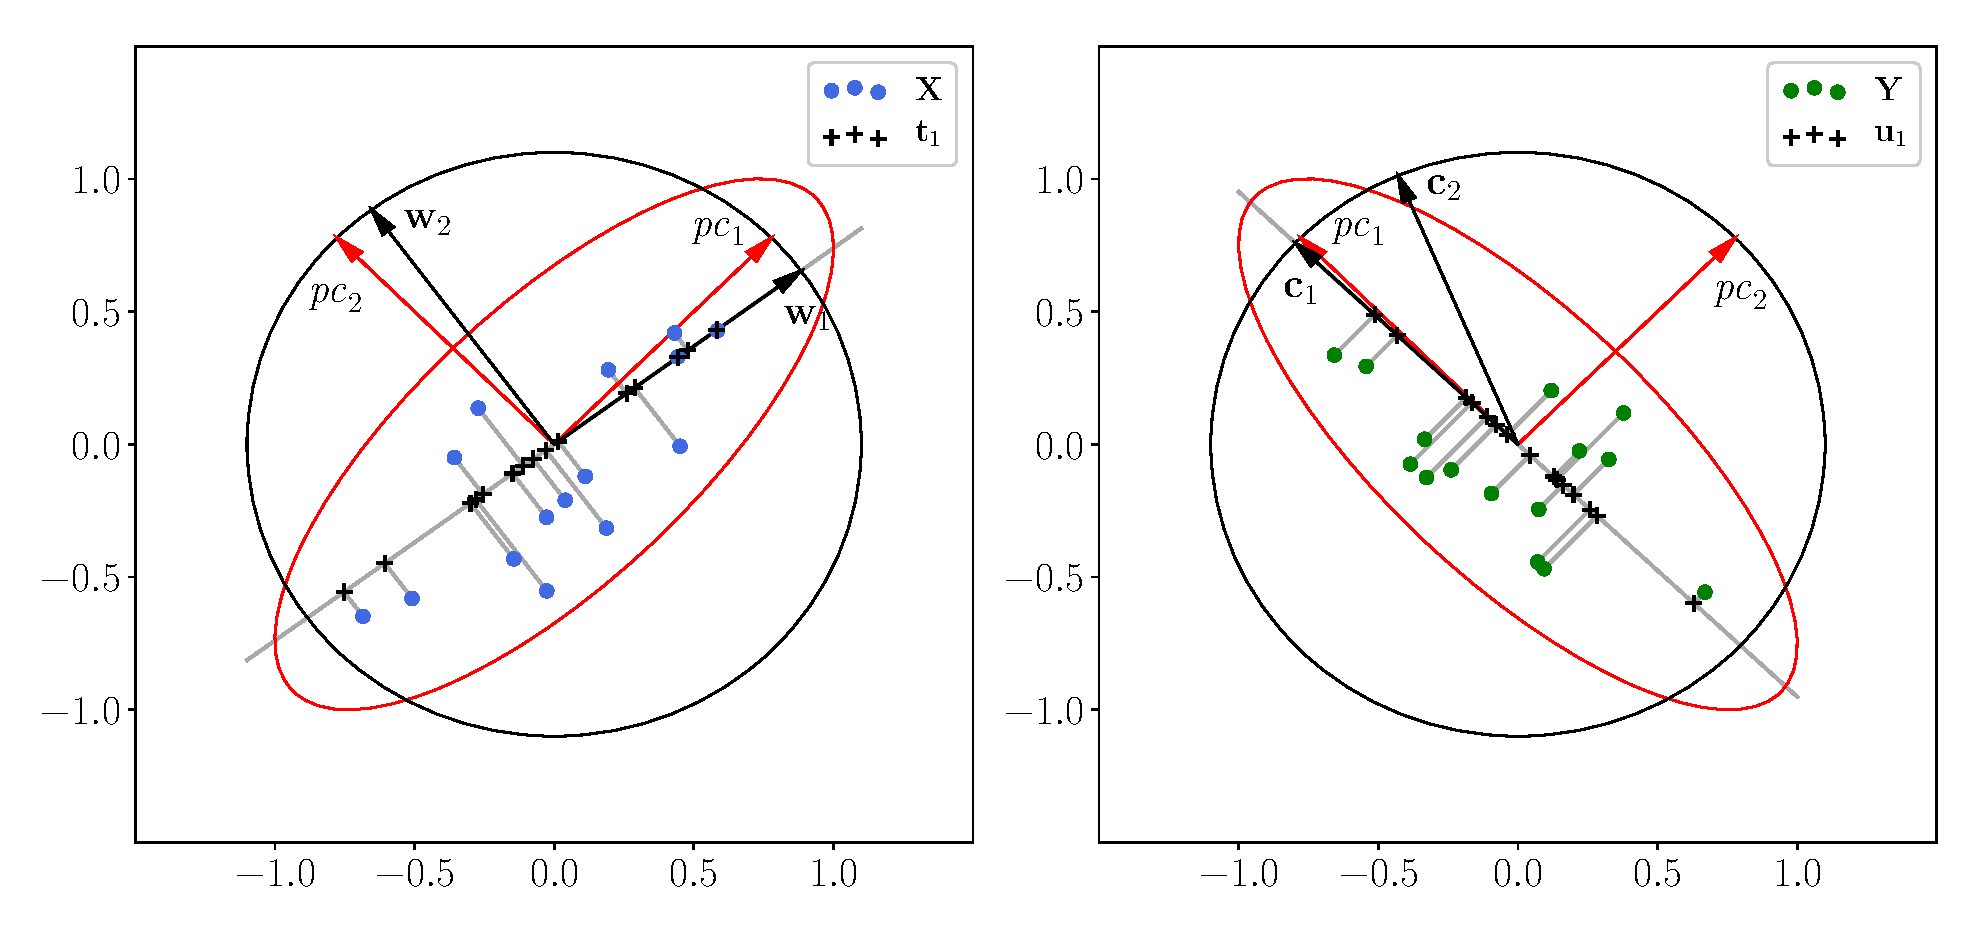
\includegraphics[width=\linewidth]{figs/PLSFigure.eps}
	\caption{The result of the PLS algorithm for the case $n = r = l = 2$}.
	\label{fig::PLSFigure}
\end{figure}

To obtain the model predictions and find the model parameters, let multiply the both hand sides of the equation~\eqref{eq::PLS_X} by the matrix $\bW$. 
Since the residual matrix  $\bE$ rows are orthogonal to the columns of the matrix $\bW$, we have
\[
	\bX \bW = \bT \bP^{\T} \bW.
\]
The linear transformation between objects in the input and latent spaces has the form
\begin{equation}
	\bT = \bX \bW^*,
	\label{eq::W*}
\end{equation}
where $\bW^* = \bW (\bP^{\T} \bW)^{-1}$.

The matrix of the model parameters~\ref{eq::model} could be found from equations~\eqref{eq::PLS_Y},~\eqref{eq::W*}
\begin{equation*}
    \bY = \bT \bQ^{\T} + \bE = \bX \bW^* \bQ^{\T} + \bE = \bX \bTheta + \bE.
\end{equation*}
Thus, the model parameters~\eqref{eq::model} are equal to
\begin{equation}
    \bTheta = \bW (\bP^{\T} \bW)^{-1} \bQ^{\T}.
    \label{eq::model_parameters}
\end{equation}

To find the model predictions during the testing we have to
\begin{itemize}
	\item normalize the test data;
	\item compute the prediction of the model using the linear transformation with the matrix $\bTheta$ from~\eqref{eq::model_parameters};
	\item perform the inverse normalization.
\end{itemize}

%%%%%%%%%%%%%%%%%%%%%%%%%%%%%%%%%%%%%%%%%%%%%%%%%%%%%%%%%%%%%%%%%%%%%%%%%%%%%%
\section{Computational experiment}
\label{sec:exper}
%%%%%%%%%%%%%%%%%%%%%%%%%%%%%%%%%%%%%%%%%%%%%%%%%%%%%%%%%%%%%%%%%%%%%%%%%%%%%%

Time series of energy consumption contain hourly records (total of 52 512 observations). 
The matrix $\bX$ row is the local history of the signal for one week $n = 24 \times 7$. 
The matrix $\bY$ row is the local forecast of energy consumption for the next 24 hours $r = 24$. 
In this case, the matrices $\bX$ and $\bY$ are autoregressive matrices.

In the ECOG data case, the matrix $\bX$ consists of the spatial-temporal representation of voltage time series, and the matrix $\bY$ contains information about the hand position.
The generation process of the matrix $\bX$ from the voltage values is described in~\cite{gasanov2017pls}. 
Feature description in each time moment has dimension equal to $864$. The hand position is described by the coordinates along three axes. 
An example of voltage data samples with the different channels and corresponding spatial coordinates of the hand are shown in Fig.~\ref{fig::ecog_data}.
To predict the hand position in the next moments we used an autoregressive approach.
One object consists of a feature description in a few moments. 
The answer is the hand position in the next moments of time.
The task is to predict the hand position in the next few moments of time.

\begin{figure}
	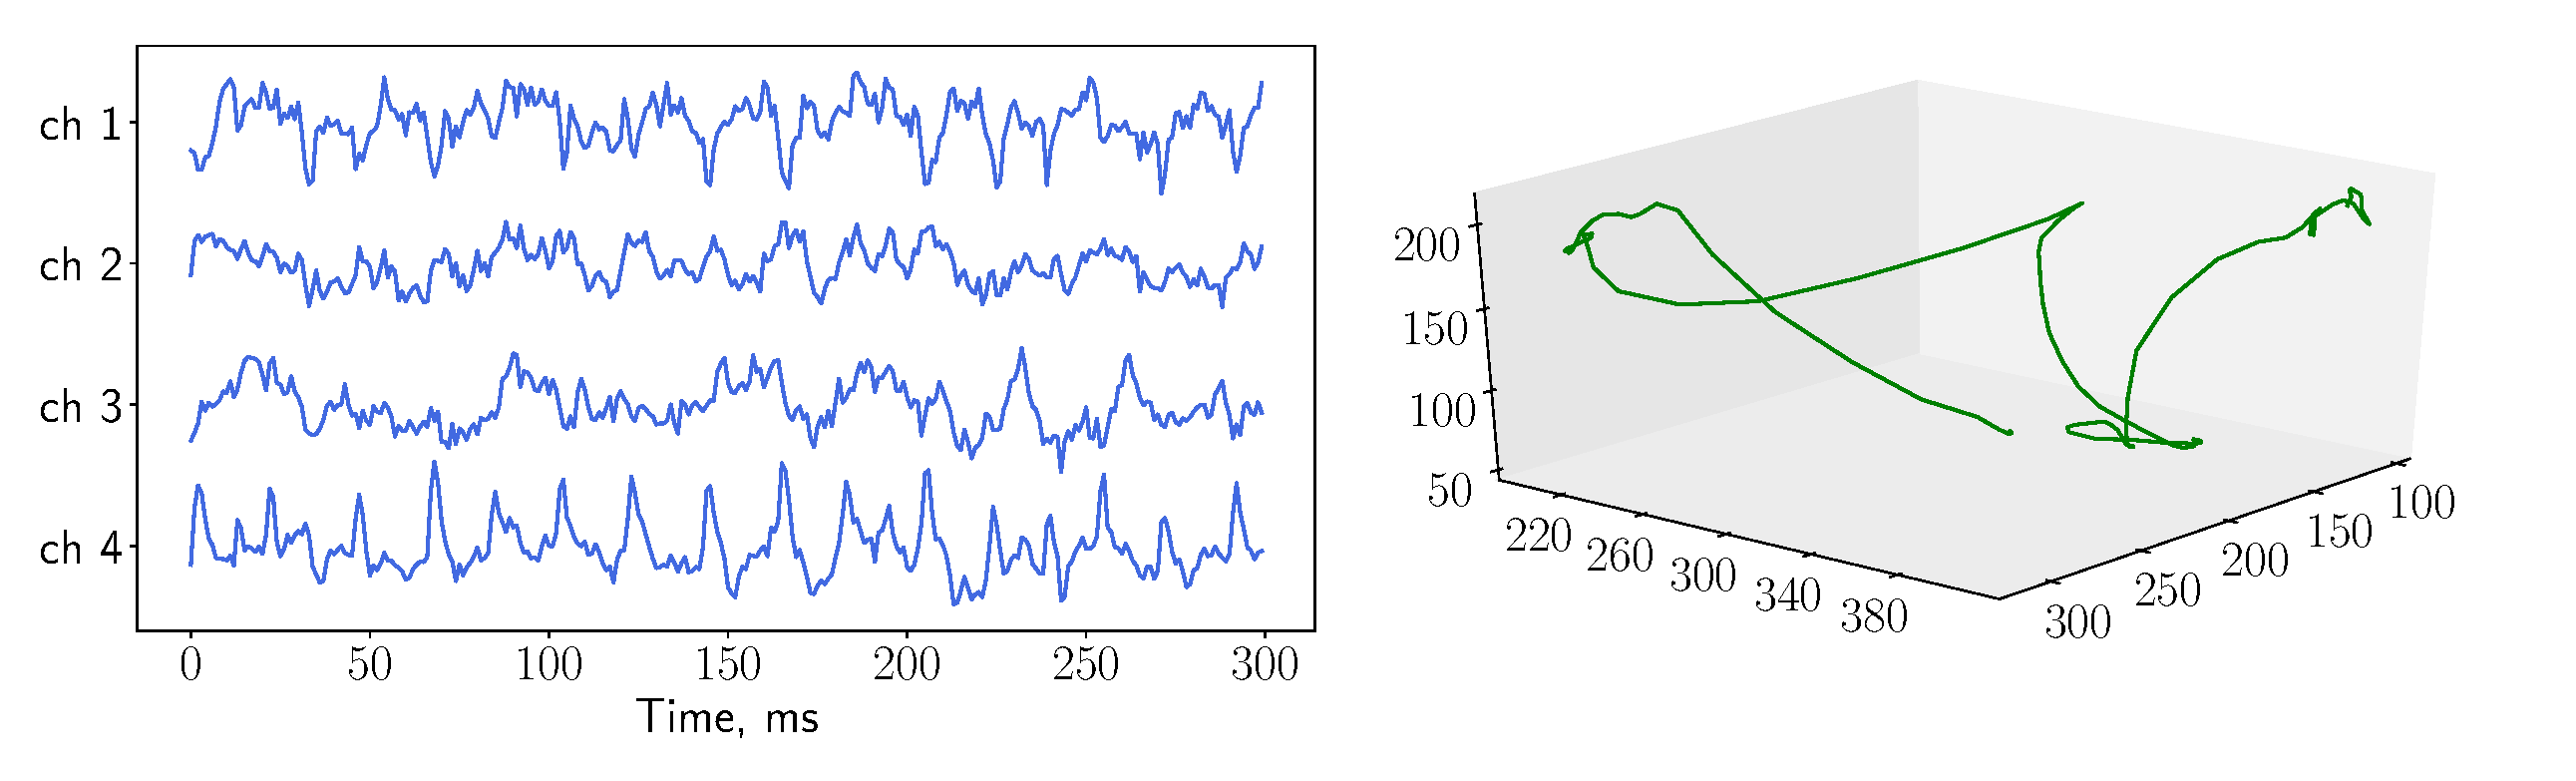
\includegraphics[width=\linewidth]{figs/ecog_data.eps}
	\caption{The ECoG data example. On the left the voltage data taken from multiple channels is shown, on the right there are coordinates of the hand along three axes.}
	\label{fig::ecog_data}
\end{figure}

We introduce the mean-squared error for matrices $\mathbf{A} = [a_{ij}]$ and $\mathbf{B} = [b_{ij}]$ 
\[
\text{MSE} (\mathbf{A}, \mathbf{B}) = \sum_{i,j} (a_{ij} - b_{ij})^2.
\]
To estimate the prediction quality, we compute the normalized MSE 
\begin{equation}
\text{NMSE}(\bY,  \mathbf{\hat{Y}}) = \frac{\text{MSE} (\bY, \mathbf{\hat{Y}})}{\text{MSE} (\bY, \mathbf{\bar{Y}})},
\label{eq::nmse}
\end{equation}
where $\mathbf{\hat{Y}}$ is the model outcome, $\mathbf{\bar{Y}}$ is the average constant forecast over the columns of the matrix.

\subsection{Energy consumption dataset}

To find the optimal dimensionality $l$ of the latent space, the energy consumption dataset was divided into training and validation parts. 
The training data consists of $700$ objects, the validation data~--- of $370$. The dependence of the normalized mean-squared error~\eqref{eq::nmse} on the latent space with dimensionality $l$ is shown in Fig.~\ref{fig::energy_n_comp}. 
First, the error drops sharply with increasing the latent space dimensionality and then changes slightly.

\begin{figure}[!h]
	\centering
	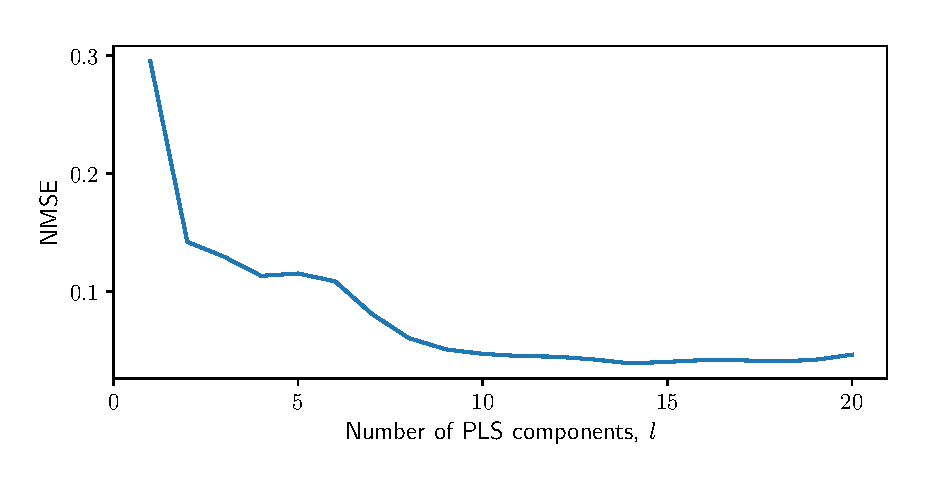
\includegraphics[width=0.75\linewidth]{figs/energy_n_comp}
	\caption{NMSE as a function of dimension $l$ of latent space for energy consumption data.}
	\label{fig::energy_n_comp}
\end{figure}

The error achieves the minimum value for $l=14$. 
Let us build a forecast of energy consumption for a given $l$. 
The result is shown in Fig.~\ref{fig::energy_prediction}. 
The PLS algorithm restored the autoregressive dependence and found the daily seasonality.

\begin{figure}[!h]
	\centering
	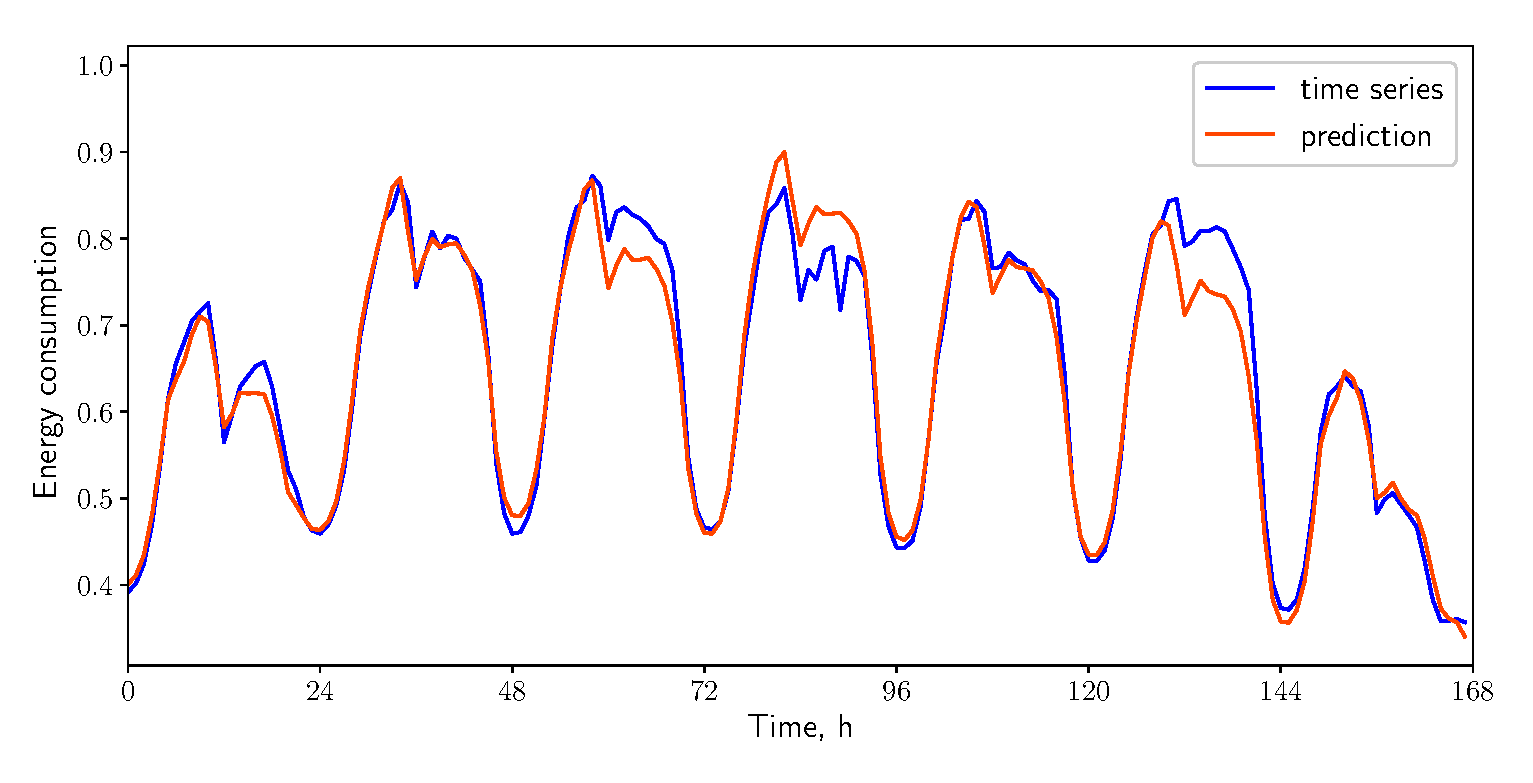
\includegraphics[width=0.95\textwidth]{figs/energy_prediction}
	\caption{The energy consumption forecast by the PLS algorithm (the latent space dimensionality is equal to $l=14$).}
	\label{fig::energy_prediction}
\end{figure}

\subsection{ECoG dataset}
Fig.~\ref{fig::ecog_n_comp} illustrates the dependence of the normalized mean-squared error~\eqref{eq::nmse} on the latent space dimensionality $l$ for ECoG dataset. 
The approximation error changes slightly for $l > 5$.
The joint spatial-temporal representation of objects and the hand position can be represented as a vector of dimensionality equal to $l \ll n$.
Let us fix $l = 5$. 
An example of the hand position approximation is shown in Fig.~\ref{fig::ecog_prediction}. 
Solid lines represent the true coordinates of the hand along all axes, the dotted lines show the approximation by the PLS algorithm.
 
\begin{figure}[!h]
	\centering
	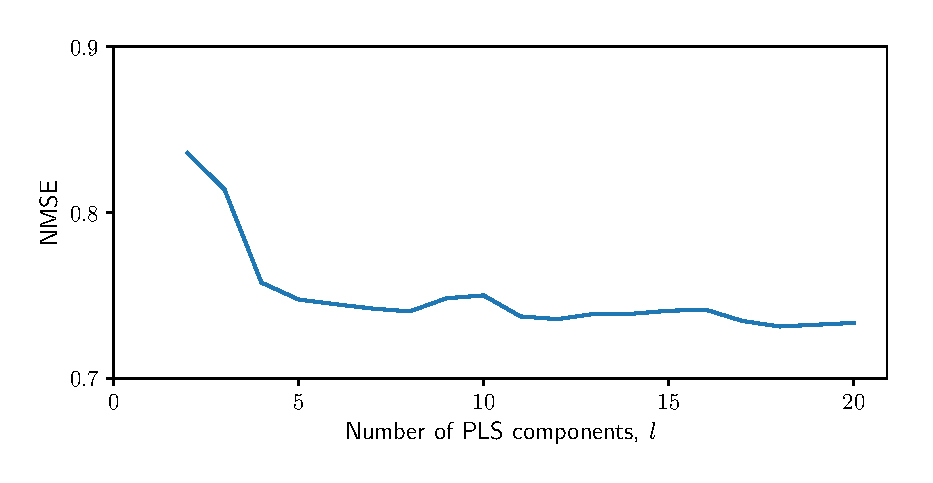
\includegraphics[width=0.75\linewidth]{figs/ecog_n_comp}	
	\caption{NMSE as a function of dimension $l$ of latent space for the ECoG data.}
	\label{fig::ecog_n_comp}
\end{figure}

\begin{figure}[!h]
	\centering
	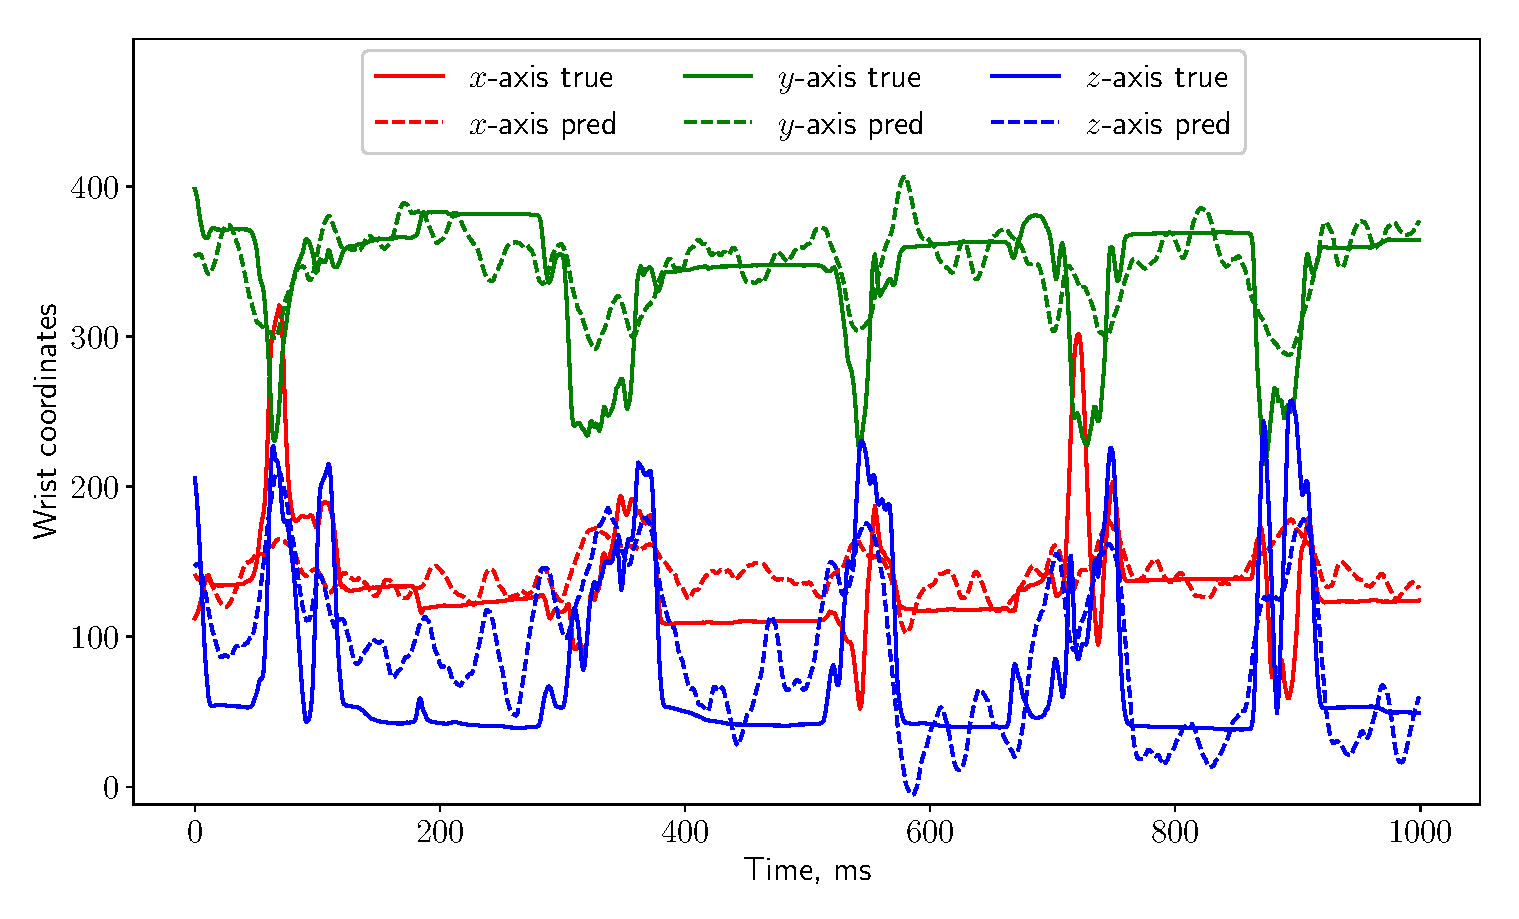
\includegraphics[width=\textwidth]{figs/ecog_prediction}
	\caption{The hand motions predicted by the PLS algorithm (the latent space dimensionality is equal to $l=5$).}
	\label{fig::ecog_prediction}
\end{figure}

%%%%%%%%%%%%%%%%%%%%%%%%%%%%%%%%%%%%%%%%%%%%%%%%%%%%%%%%%%%%%%%%%%%%%%%%%%%%%%
\section{Conclusion}
In the paper we proposed the approach for solving the problem of time series decoding and forecasting. 
The algorithm of partial least squares allows to build a simple, stable, and linear model. 
The obtained latent space gathers information about the objects and the responses and dramatically reduces the dimensionality of the input matrices. 
The computational experiment demonstrated the proposed method applicability to the tasks of electricity consumption forecasting and brain-computer interface designing.
The future research will be aimed to the extension of the proposed method for the non-linear dependencies class.
%%%%%%%%%%%%%%%%%%%%%%%%%%%%%%%%%%%%%%%%%%%%%%%%%%%%%%%%%%%%%%%%%%%%%%%%%%%%%%

\bibliographystyle{unsrt}
\bibliography{papers_pls}


\end{document}